\documentclass{ieeeaccess}
\usepackage{cite}
\usepackage{amsmath,amssymb,amsfonts}
\usepackage{algorithmic}
\usepackage{graphicx}
\usepackage{textcomp}
\usepackage{hyperref}

\usepackage{bm}
\makeatletter
\AtBeginDocument{\DeclareMathVersion{bold}
\SetSymbolFont{operators}{bold}{T1}{times}{b}{n}
\SetSymbolFont{NewLetters}{bold}{T1}{times}{b}{it}
\SetMathAlphabet{\mathrm}{bold}{T1}{times}{b}{n}
\SetMathAlphabet{\mathit}{bold}{T1}{times}{b}{it}
\SetMathAlphabet{\mathbf}{bold}{T1}{times}{b}{n}
\SetMathAlphabet{\mathtt}{bold}{OT1}{pcr}{b}{n}
\SetSymbolFont{symbols}{bold}{OMS}{cmsy}{b}{n}
\renewcommand\boldmath{\@nomath\boldmath\mathversion{bold}}}
\makeatother

\def\BibTeX{{\rm B\kern-.05em{\sc i\kern-.025em b}\kern-.08em
    T\kern-.1667em\lower.7ex\hbox{E}\kern-.125emX}}

%Your document starts from here ___________________________________________________

\graphicspath{ {./images/} }

\begin{document}
\history{Date of publication xxxx 00, 0000, date of current version xxxx 00, 0000.}
\doi{10.1109/ACCESS.2024.0429000}

\title{Refining Software Clustering: The Impact of Code Co-Changes on Architectural Reconstruction}
\author{\uppercase{Stana Adelina Diana}\authorrefmark{1} and
\uppercase{Sora Ioana}\authorrefmark{2}
}

\address[1]{Computer Science and Engineering Department
”Politehnica” University of Timisoara, Romania (e-mail: stana.adelina.diana@gmail.com)}
\address[2]{Computer Science and Engineering Department
”Politehnica” University of Timisoara, Romania (e-mail: ioana.sora@cs.upt.ro)}

\markboth
{Author \headeretal: Preparation of Papers for IEEE TRANSACTIONS and JOURNALS}
{Author \headeretal: Preparation of Papers for IEEE TRANSACTIONS and JOURNALS}

\corresp{Corresponding author: Stana Adelina Diana (e-mail: stana.adelina.diana@gmail.com).}


\begin{abstract}
Version control systems primarily offer support for tracking and managing changes in software code, but they can also provide a great deal of additional information about the managed software. Changes in multiple software entities simultaneously can imply that these entities are connected to one another. Software entities that change at the same time (code co-changes) are treated as a distinct category of software dependencies. In some cases, these co-changes are used together with other types of dependencies, such as structural dependencies or lexical dependencies, to enhance the understanding of a software system.


This paper proposes using code co-changes in software clustering for architectural reconstruction. Structural dependencies are the most commonly used type of dependencies in software clustering for architectural reconstruction, so we will use clustering solutions obtained from structural dependencies as the baseline for our evaluations. Our approach will be applied to four open-source projects found on GitHub. For each of the projects, we will compare and evaluate the clustering obtained by using only co-changes and the clustering obtained by using co-changes combined with structural dependencies with the baseline clustering generated solely from structural dependencies.
\end{abstract}

\begin{keywords}
Architectural reconstruction, code co-changes, logical dependencies, software clustering, software dependencies, versioning system.
\end{keywords}

\titlepgskip=-21pt

\maketitle

\section{Introduction}
\label{sec:introduction}

Software systems often face a lack of documentation. Even if there was original documentation at the beginning of development, over the years it may become outdated or lost. Additionally, the original developers may leave the company, taking with them knowledge about how the software was designed. This situation challenges the teams when it comes to maintenance or modernization. In this context, recovering the system's architecture is essential. Understanding the system's architecture helps developers better evaluate and understand the nature and impact of changes they need to make. One technique to aid in reconstructing the system architecture is software clustering. Software clustering involves creating cohesive groups (modules) of software entities based on their dependencies and interactions.

Among the dependencies that can be used for software clustering are structural dependencies (relationships between entities based on code analysis), lexical dependencies (relationships based on naming conventions), and code co-changes/logical dependencies (relationships between entities extracted from the version control system), among others. Combining multiple types of dependencies, rather than relying on just one type, can be a good approach to generate better results. However, it requires fine-tuning the amount of dependencies used from each category and scaling the coefficients attached to them. Combining dependencies without considering these aspects might lead to results that are less effective than using an individual type of dependency alone.

In this paper, we assess whether using structural dependencies combined with logical dependencies can provide better results than using each type of dependency alone. The structural dependencies are used as they are extracted from static code analysis. The logical dependencies are filtered co-changes from the version control system. The reason behind filtering the co-changes and not using them as they are in the versioning system is to enhance their quality and make them easier to combine with structural dependencies, as their size can outnumber the structural dependencies \cite{b1}.

To evaluate the results, we generate software clustering on four open-source projects and use two types of metrics for comparison. One of the metrics is MQ (Modularization Quality), which evaluates the modularization quality based on the interaction between the modules and does not require any additional input besides the clustering result \cite{b2}. The other is the MoJo (Move and Join) metric, a commonly used metric for evaluating the similarity between two different software clustering results \cite{b3}. For this metric, we manually generate a base of comparison for the clustering result and compare it against this baseline.

In Section \ref{sec:related_work}, we review the related work and previous studies that used various dependencies for software clustering and their metrics for evaluation.
Section \ref{sec:workflow_implementation} details the workflow and implementation of our approach, including the extraction and filtering of dependencies, and the clustering algorithm used.
The results of our experiments on four open-source projects are presented in Section \ref{sec:results}. Section \ref{sec:evaluation} evaluates our results by using the Modularization Quality (MQ) metric and the Move and Join (MoJo) metric. We also manually analyze some of the clustering solutions.
Finally, Section \ref{sec:conclusion} contains our conclusions, findings, and potential directions for future work.

\subsection{Abbreviations and Acronyms}

The following abbreviations and acronyms are used throughout this article:

\begin{itemize}
    \item \textbf{LD}: Logical Dependencies
    \item \textbf{SD}: Structural Dependencies
    \item \textbf{MQ}: Modularization Quality Metric
    \item \textbf{MoJo}: Move and Join Metric
\end{itemize}


Logical Dependencies (LD) refer to the relationships between software entities that have been extracted and filtered from the versioning system. If these entities are not filtered, they are simply referred to as co-changes. 
Structural Dependencies (SD), on the other hand, refer to the relationships between software entities extracted from static code analysis.
Modularization Quality Metric (MQ) and Move and Join Metric (MoJo) are metrics used to evaluate software clustering results.

\section{Related Work}
\label{sec:related_work}


\section{Workflow and Implementation}
\label{sec:workflow_implementation}


To achieve our goal of evaluating how the quality of clustering solutions is impacted by logical dependencies, we developed a Python tool capable of using any type of dependency, either alone or combined with other types of dependencies, as long as they are provided in CSV format. The tool clusters and evaluates software clustering solutions using either the MQ metric or the MoJo metric. In the following subsections, we present how we obtain the structural dependencies and logical dependencies used, the type of clustering algorithm we use, and the tool's workflow.

\subsection{Structural Dependencies}
\label{subsec:sd}

The structural dependencies are obtained using a tool from our previous research. While the tool primarily exports the key class ranking of a software system, it also has the capability to export the data in CSV format. The exported dependencies are directed and weighted based on the type of dependency they represent.

\subsection{Logical Dependencies}
\label{subsec:ld}

We refer to logical dependencies as the filtered co-changes between software entities. A co-change occurs when two or more software entities are modified together during the same commit in the version control system. Co-changes indicate that these entities are likely related or dependent on each other, directly or indirectly.

There is a degree of uncertainty associated with co-changes. Compared to structural dependencies, where the presence of a dependency is certain, co-changes are less reliable. For example, if the system was migrated from one version control system to another, the first commit will include all the entities from the system at that point in time. Should we consider all these entities as related to one another in this case? This would introduce false dependencies and reduce the likelihood of achieving accurate results when combining them with more reliable types of dependencies.

Even if we address the issue of the first commit, it can still happen that a developer resolves multiple unrelated issues in the same commit (even though this is not recommended by development processes).

To solve this problem, in our previous works, we refined some filtering methods to ensure that the co-changes that remain after filtering are more reliable and suitable for use with other dependencies or individually \cite{b4}, \cite{b5}, \cite{b6}. Based on our previous results, the filters we decided to use further in our research are the commit size filter and the strength filter. Both filters are used together, and the end result is the set of logical dependencies that we use to generate software clusters.

\subsubsection{Commit Size Filter}

The commit size filter filters out all co-changes that originate from commits that exceed a certain number of files.

We are interested in extracting dependencies from code commits that involve feature development or bug fixes because that is when developers change related code files. If multiple unrelated features or bug fixes are solved in a single commit, it will appear as though all the entities in those files are related, even if they are not.

One scenario where this issue arises is the first commit of a software system when it is ported from one versioning system to another. This commit will contain many changed code files, but these changes do not originate from any functionality change, so they generate numerous irrelevant co-changes for the system.

A similar scenario occurs with merge commits. A merge commit is created automatically when you perform a merge operation to integrate changes from one branch into another. After integration, all commits from the branch are added to the target branch, and on top of that, there is the merge commit containing all changes from the commits merged into a single commit. Since this commit contains only a merge of multiple smaller, related issues/features solved, it is better to gather information from the smaller commits rather than from the overall merge commit.

What both scenarios above have in common is the large number of files involved in the commits. Based on our previous research and measurements regarding the number of files involved in a commit, we chose to set a threshold of 10 files \cite{b4}, \cite{b5}. Therefore, all co-changes that originate from commits with more than 10 changed code files are filtered out.

\subsubsection{Strength Filter}

This filter focuses on the reliability of the co-changes. If a pair of co-changing entities appears only once in the entire history of the system, it might be less reliable than a pair that appears more frequently.

Zimmermann et al. introduced the support and confidence metrics to measure the significance of co-changes \cite{b7}.

The \textit{support metric} of a rule $(A \rightarrow B)$ where A is the antecedent and B is the consequent of the rule, is defined as the number of commits (transactions) in which both entities are changed together.

The \textit{confidence metric} of $(A \rightarrow B)$, as defined in Equation \eqref{eq:confidence} , focuses on the antecedent of the rule and is the number of commits together of both entities divided by the total number of commits of (A).


\begin{equation}
\text{Confidence}(A \rightarrow B) = \frac{\text{Nr. of commits containing } A \text{ and } B}{\text{Nr. of commits containing } A}
\label{eq:confidence}
\end{equation}


The confidence metric favors entities that change less and more frequently together, rather than entities that change more with a wider variation of other entities.

Assuming that (A) was changed in 10 commits and, of these 10 commits, 9 also included changes to (B), the confidence for the rule $(A \rightarrow B)$ is 0.9. On the other hand, if (C) was changed in 100 commits and, of these 100 commits, 50 also included changes to (D), the confidence for the rule $(C \rightarrow D)$ is 0.5. Therefore, in this scenario, we would have more confidence in the first pair $(A \rightarrow B)$ than in the second pair $(C \rightarrow D)$, even though the second pair has more than five times more updates together.

To favor entities that are involved in more commits together, we calculated a \textit{system factor}. This system factor is the mean value of the support metric values for all entity pairs.

The system factor is multiplied with the calculated confidence metric value. In addition, since we plan to use the metric values as weights, together with the weights of the structural dependencies, we multiply by 100 to scale the metric value to be supraunitary, and we clip the results between 0 and 100.


We refer to this addition to the original calculation formula as strength metric, and it is defined in Equation \eqref{eq:strength}.

\begin{equation}
\text{strength}(A \rightarrow B) = \text{confidence}(A \rightarrow B) \times 100 \times \text{system factor} 
\label{eq:strength}
\end{equation}


\subsubsection{Filter Application Process}

The overall filter application process is illustrated in Fig. \ref{fig:filtering}.  We begin by extracting all co-changes from the versioning system, and the first filter applied is the commit size filter. The commit size filter has a strict threshold of 10 files, meaning that any co-changes from commits involving more than 10 files are filtered out.

The co-changes that remain after applying the commit size filter are then processed using the strength filter. The strength filter uses multiple thresholds, specifically 10 different thresholds. We start with a threshold of 10 and increment it by 10 until we reach a maximum value of 100. The reason for not using a fixed threshold is to assess how different strength thresholds affect our cluster generation. 

\begin{figure}[t!]
  \centering
  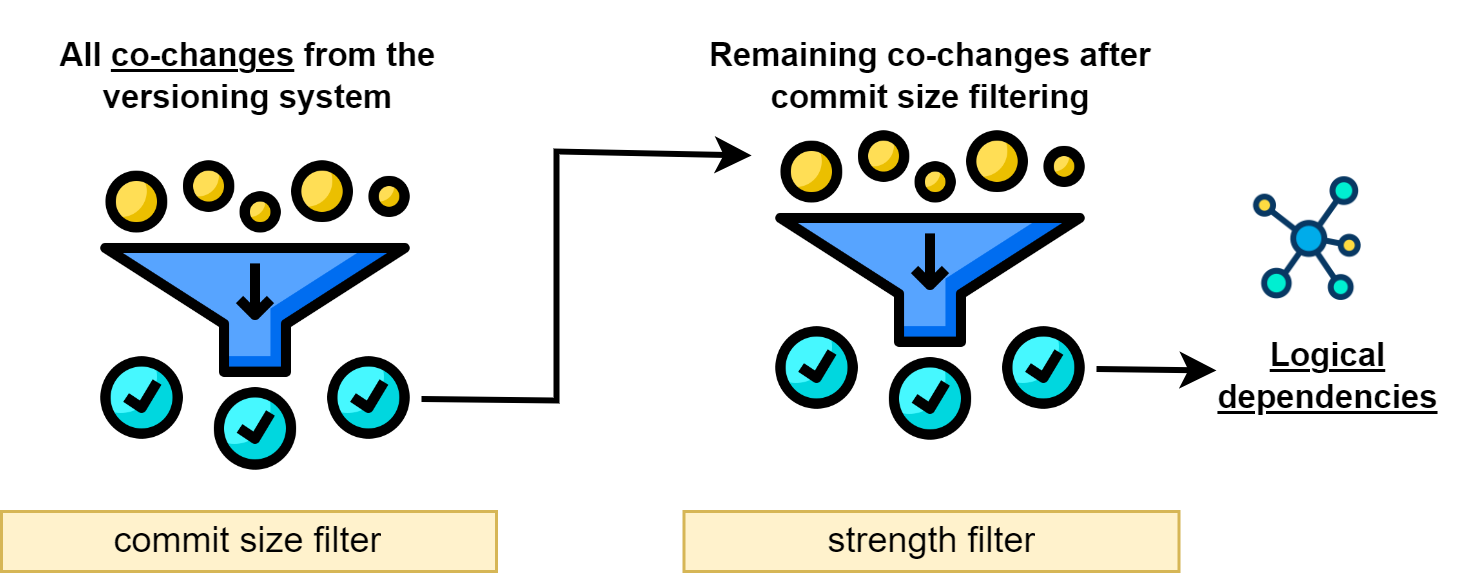
\includegraphics[width=\columnwidth]{filtering.png}
  \caption{ \textbf{Filter application process}}
  \label{fig:filtering}
\end{figure}

To extract and filter the co-changes, we used a previously developed tool \cite{b4}. This tool takes as input the GitHub repository address and the threshold values for commit and strength filters. The tool clones the repository, downloads all commit diffs starting from the first commit, examines all files changed in each commit to identify which entities have changed in those files, and creates undirected co-change dependencies between all changed entities within a commit.

The commit size filter is applied to these undirected co-change dependencies, since the metric value for $(A \rightarrow B)$ is the same as for $(B \rightarrow A)$. For the strength filter, each co-change dependency is converted into a directed co-change dependency, so for each $(A \rightarrow B)$ dependency we have both $(A \rightarrow B)$ and $(B \rightarrow A)$. This conversion is necessary because, as mentioned in the previous section, the confidence filter, upon which the strength filter is built, evaluates the antecedent of the rule. Thus, the metric value for $(A \rightarrow B)$ differs from the metric value for $(B \rightarrow A)$.

The remaining dependencies after applying the strength filter are then exported to a CSV file for further use.

\Figure[t!](topskip=0pt, botskip=0pt, midskip=0pt)[width=\textwidth]{workflow-tool.png}
{ \textbf{Tool workflow overview: input, processing and output.}\label{fig:tool}}

\subsection{Louvain Clustering Algorithm}
\label{subsec:louvain}

The Louvain algorithm was originally developed by Blondel et al. and is used for finding community partitions (clusters) in large networks. The algorithm begins with a weighted network of N nodes, initially assigning each node to its own cluster, resulting in N clusters. For each node, the algorithm evaluates the modularity gain from moving the node to the cluster of each of its neighbors. Based on the results, the node is moved to the cluster with the maximum positive modularity gain. This process is repeated for all nodes until no further improvement in modularity is possible \cite{b8}.

The modularity of a cluster is a value that ranges from -1 to 1, which measures the density of connections inside clusters compared to connections between clusters \cite{b9}.


\subsection{Clustering result evaluation}
\label{subsec:evaluation_def}

\subsubsection{Modularity Quality Metric}

\subsubsection{MoJo Metric}

\subsection{Tool Workflow Overview}
\label{subsec:tool_workflow}

To generate the cluster solutions and evaluate the results, we created a tool in Python. The entire workflow of the tool is presented in Fig. \ref{fig:tool}.

\subsubsection{Input}

The tool takes as input one or multiple dependency CSV files and the baseline solution required for the MoJo metric. We designed the tool to accept multiple dependency files so that we can generate clustering solutions based on either a single type of dependency (structural or logical) or a combination of both.

Since the MoJo metric requires a baseline solution to evaluate the generated solution, we manually inspected the code and created baseline clustering solutions, which we then provide as input for the tool.

\subsubsection{Processing}

The dependencies are saved in the CSV file in the following format: antecedent of a dependency, consequent of a dependency, weight. The tool reads each line, adds the antecedent and consequent as nodes in a directed graph, and creates an edge between them, with the weight from the CSV file becoming the edge weight. If multiple dependency files are processed and the same dependency is found in multiple files, the edge weights are summed.


After all dependencies are read, the directed graph is passed to the Louvain clustering algorithm to generate the clustering result. The clustering result is then evaluated. The MQ metric requires the directed graph and the clustering result, while the MoJo metric requires the baseline clustering solution provided as input and the clustering result.

\subsubsection{Output}

After both evaluations are done, we export the clustering result, the cluster count, and the values for both metrics.

\section{Results}
\label{sec:results}

To assess the impact of using logical dependencies in software clustering, we run the tool presented in Section \ref{subsec:tool_workflow} in three different scenarios. All three scenarios are illustrated in Fig. \ref{fig:scenatrio}.

In the first scenario, we run the tool once, providing only the structural dependencies of the system as input for the clustering algorithm.

In the second scenario, we run the tool ten times, using only logical dependencies as input. We perform ten runs because we generate logical dependencies with different threshold values for the strength filter. We start with a threshold of 10 and increase it in steps of 10 up to 100.

In the third scenario, we combine logical with structural dependencies. Again, we run the tool ten times, each time using structural dependencies and logical dependencies generated with different strength thresholds.

\begin{figure}[t!]
  \centering
  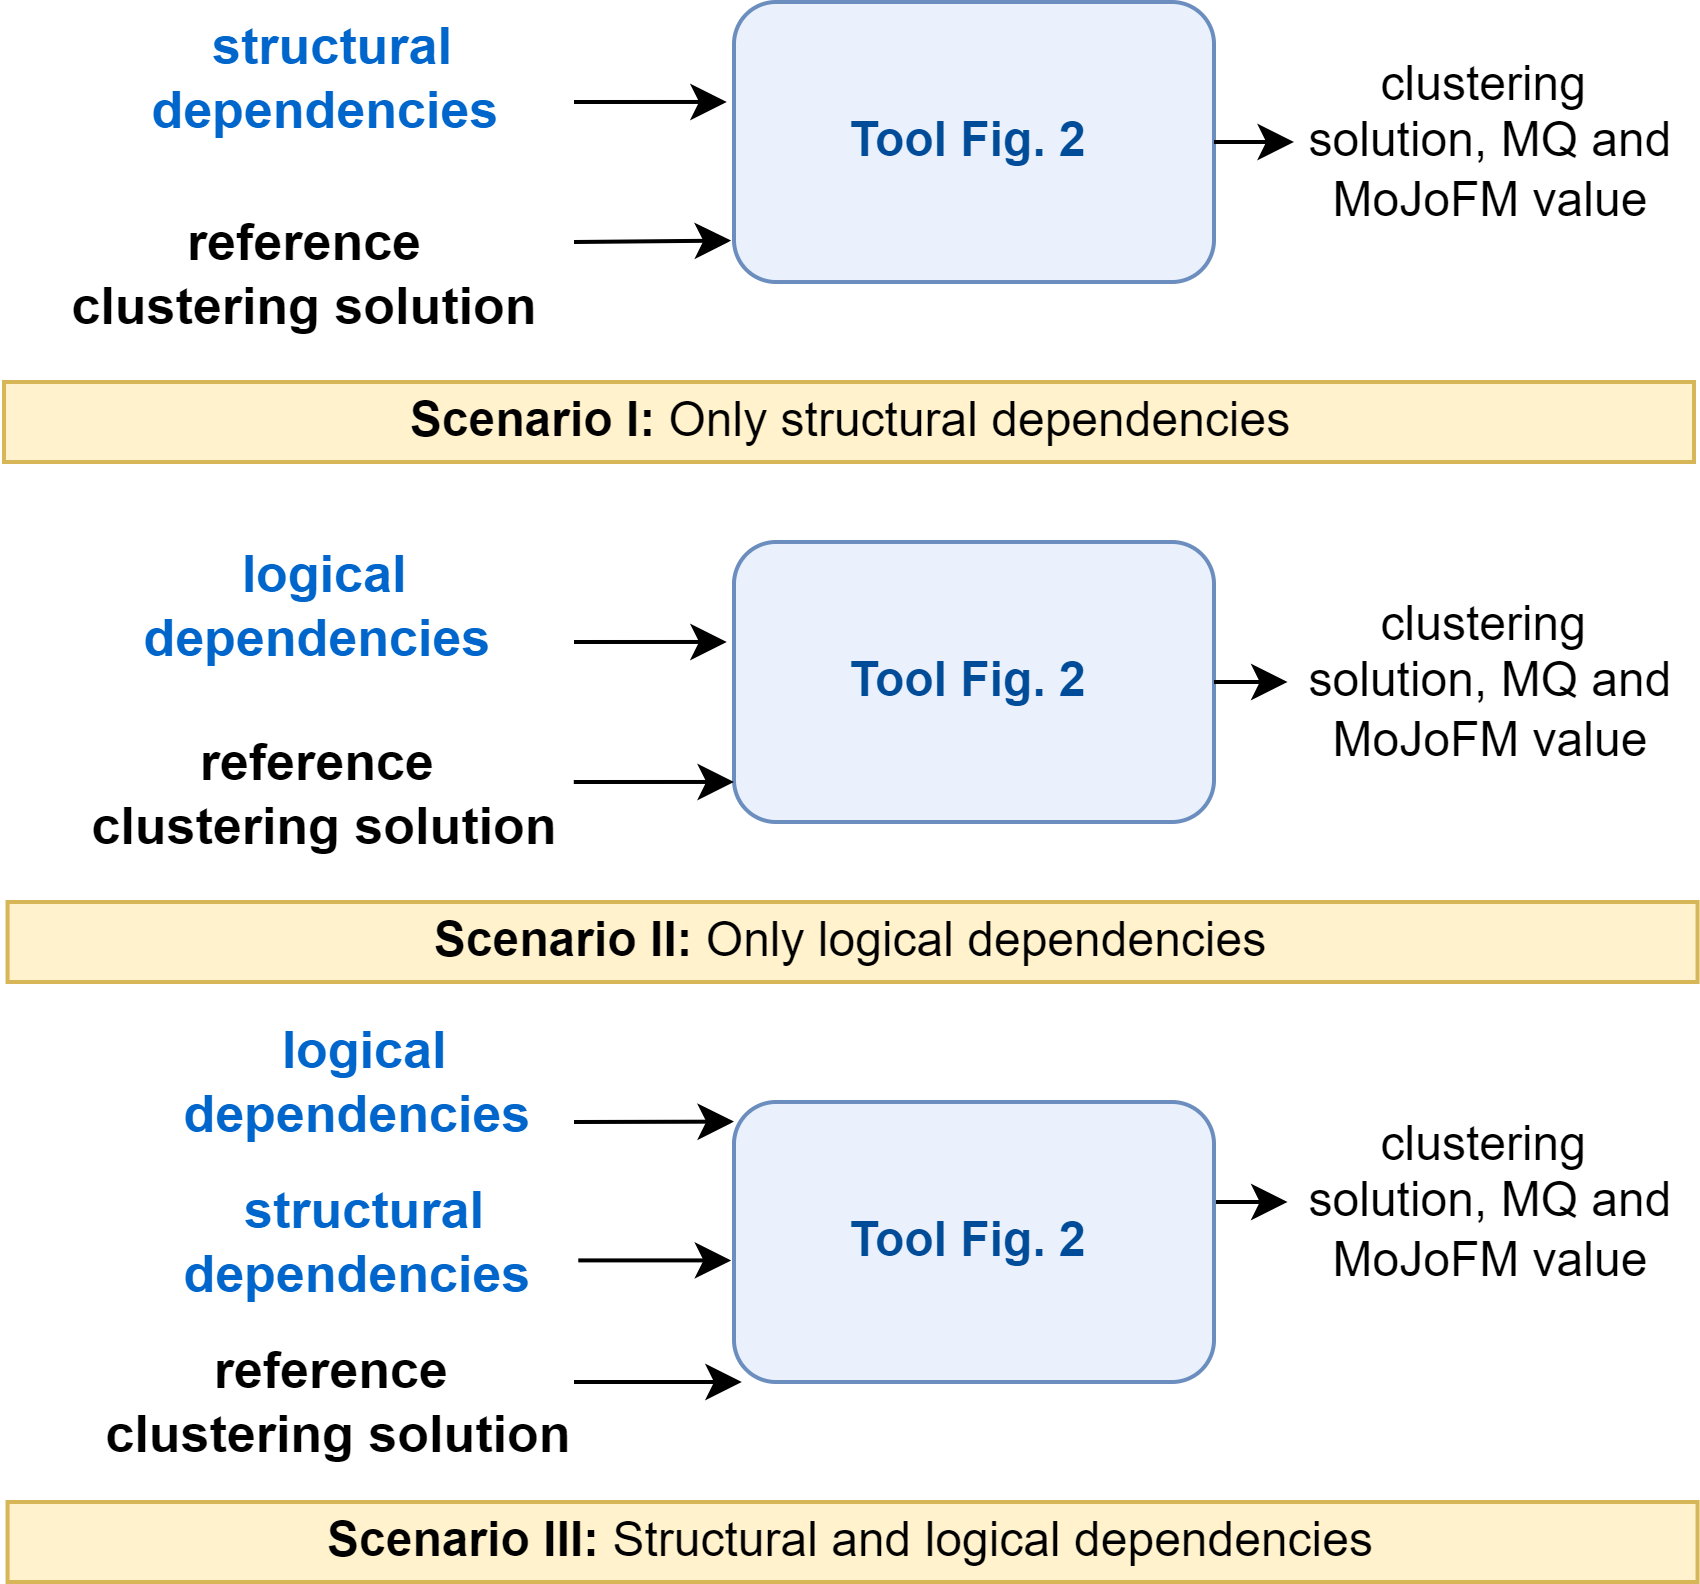
\includegraphics[width=\columnwidth]{scenario.png}
  \caption{ \textbf{Scenarios for results}}
  \label{fig:scenatrio}
\end{figure}

\begin{table}[h]
\caption{Clustering Results Based on Different Dependency Types And Strength Filter Thresholds For Repo: \url{https://github.com/apache/ant}}
\label{tab:clustering_results_ant}
\centering
\setlength{\tabcolsep}{10pt}
\begin{tabular}{|l|c|c|c|c|}
\hline
\textbf{Dependency Type} & \textbf{Nr. Of} & \textbf{Class} & \textbf{MQ} & \textbf{Mojo} \\
\textbf{[Strength thresh.]} & \textbf{clusters} & \textbf{Count} &  &  \\
\hline
\textbf{SD} & \textbf{14} & \textbf{517} & \textbf{0.085} & \textbf{181} \\
LD [10] & 56 & 320 & 0.047 & 301 \\
LD [20] & 53 & 215 & 0.040 & 361 \\
LD [30] & 44 & 174 & 0.036 & 384 \\
LD [40] & 40 & 152 & 0.034 & 401 \\
LD [50] & 35 & 138 & 0.030 & 407 \\
LD [60] & 34 & 120 & 0.029 & 423 \\
LD [70] & 32 & 106 & 0.027 & 432 \\
LD [80] & 29 & 92 & 0.024 & 443 \\
LD [90] & 24 & 79 & 0.021 & 451 \\
LD [100] & 19 & 64 & 0.019 & 461 \\
\hline
SD+LD [10] & 15 & 517 & 0.087 & 173 \\
SD+LD [20] & 13 & 517 & 0.071 & 184 \\
SD+LD [30] & 13 & 517 & 0.071 & 184 \\
SD+LD [40] & 13 & 517 & 0.071 & 184 \\
SD+LD [50] & 13 & 517 & 0.071 & 184 \\
SD+LD [60] & 13 & 517 & 0.071 & 184 \\
SD+LD [70] & 13 & 517 & 0.071 & 184 \\
SD+LD [80] & 13 & 517 & 0.071 & 184 \\
SD+LD [90] & 13 & 517 & 0.071 & 184 \\
SD+LD [100] & 13 & 517 & 0.072 & 184 \\
\hline
\end{tabular}
\end{table}


\begin{table}[h]
\caption{Clustering Results Based on Different Dependency Types And Strength Filter Thresholds for Repo: \href{https://github.com/apache/tomcat}{https://github.com/apache/tomcat}}
\label{tab:clustering_results_tomcat}
\centering
\setlength{\tabcolsep}{10pt}
\begin{tabular}{|l|c|c|c|c|}
\hline
\textbf{Dependency Type} & \textbf{Nr. of} & \textbf{Class} & \textbf{MQ} & \textbf{Mojo} \\
\textbf{[Strength Thresh.]} & \textbf{Clusters} & \textbf{Count} &  &  \\
\hline
\textbf{SD} & \textbf{31} & \textbf{662} & \textbf{0.184} & \textbf{220} \\
LD [10] & 41 & 415 & 0.023 & 314 \\
LD [20] & 46 & 308 & 0.026 & 425 \\
LD [30] & 46 & 250 & 0.024 & 460 \\
LD [40] & 42 & 209 & 0.022 & 488 \\
LD [50] & 44 & 199 & 0.023 & 499 \\
LD [60] & 45 & 178 & 0.024 & 521 \\
LD [70] & 45 & 165 & 0.024 & 531 \\
LD [80] & 36 & 127 & 0.020 & 557 \\
LD [90] & 32 & 116 & 0.018 & 564 \\
LD [100] & 30 & 110 & 0.018 & 568 \\
\hline
SD+LD [10] & 26 & 662 & 0.164 & 250 \\
SD+LD [20] & 28 & 662 & 0.170 & 222 \\
SD+LD [30] & 27 & 662 & 0.166 & 221 \\
SD+LD [40] & 28 & 662 & 0.169 & 221 \\
SD+LD [50] & 28 & 662 & 0.170 & 222 \\
SD+LD [60] & 28 & 662 & 0.169 & 224 \\
SD+LD [70] & 26 & 662 & 0.173 & 232 \\
SD+LD [80] & 29 & 662 & 0.171 & 223 \\
SD+LD [90] & 29 & 662 & 0.171 & 223 \\
SD+LD [100] & 29 & 662 & 0.171 & 223 \\
\hline
\end{tabular}
\end{table}

\begin{table}[h]
\caption{Clustering Results Based on Different Dependency Types And Strength Filter Thresholds for Repo: \href{https://github.com/hibernate/hibernate-orm}{https://github.com/hibernate/hibernate-orm}}
\label{tab:clustering_results_hibernate}
\centering
\setlength{\tabcolsep}{10pt}
\begin{tabular}{|l|c|c|c|c|}
\hline
\textbf{Dependency Type} & \textbf{Nr. of} & \textbf{Class} & \textbf{MQ} & \textbf{Mojo} \\
\textbf{[Strength Thresh.]} & \textbf{Clusters} & \textbf{Count} &  &  \\
\hline
\textbf{SD} & \textbf{26} & \textbf{4414} & \textbf{0.073} & \textbf{2668} \\
LD [10] & 46 & 1469 & 0.004 & 3992 \\
LD [20] & 64 & 1343 & 0.004 & 3991 \\
LD [30] & 68 & 1242 & 0.004 & 3996 \\
LD [40] & 87 & 933 & 0.005 & 4020 \\
LD [50] & 90 & 917 & 0.005 & 4020 \\
LD [60] & 89 & 866 & 0.005 & 4074 \\
LD [70] & 93 & 474 & 0.005 & 4108 \\
LD [80] & 96 & 465 & 0.005 & 4117 \\
LD [90] & 97 & 447 & 0.005 & 4128 \\
LD [100] & 86 & 370 & 0.005 & 4174 \\
\hline
SD+LD [10] & 30 & 4414 & 0.070 & 2596 \\
SD+LD [20] & 29 & 4414 & 0.073 & 2577 \\
SD+LD [30] & 29 & 4414 & 0.073 & 2606 \\
SD+LD [40] & 29 & 4414 & 0.079 & 2648 \\
SD+LD [50] & 29 & 4414 & 0.079 & 2649 \\
SD+LD [60] & 30 & 4414 & 0.078 & 2625 \\
SD+LD [70] & 30 & 4414 & 0.072 & 2559 \\
SD+LD [80] & 30 & 4414 & 0.072 & 2559 \\
SD+LD [90] & 30 & 4414 & 0.072 & 2559 \\
SD+LD [100] & 30 & 4414 & 0.072 & 2559 \\
\hline
\end{tabular}
\end{table}


\begin{table}[h]
\caption{Clustering Results Based on Different Dependency Types And Strength Filter Thresholds for Repo: \href{https://github.com/google/gson}{https://github.com/google/gson}}
\label{tab:clustering_results_gson}
\centering
\setlength{\tabcolsep}{10pt}
\begin{tabular}{|l|c|c|c|c|}
\hline
\textbf{Dependency Type} & \textbf{Nr. of} & \textbf{Class} & \textbf{MQ} & \textbf{Mojo} \\
\textbf{[Strength Thresh.]} & \textbf{Clusters} & \textbf{Count} &  &  \\
\hline
\textbf{SD} & \textbf{10} & \textbf{210} & \textbf{0.144} & \textbf{83} \\
LD [10] & 10 & 67 & 0.018 & 164 \\
LD [20] & 11 & 50 & 0.022 & 177 \\
LD [30] & 12 & 41 & 0.027 & 182 \\
LD [40] & 8 & 31 & 0.022 & 186 \\
LD [50] & 8 & 31 & 0.022 & 186 \\
LD [60] & 8 & 28 & 0.021 & 189 \\
LD [70] & 7 & 26 & 0.018 & 190 \\
LD [80] & 5 & 18 & 0.014 & 196 \\
LD [90] & 5 & 18 & 0.014 & 196 \\
LD [100] & 5 & 18 & 0.014 & 196 \\
\hline
SD+LD [10] & 10 & 210 & 0.144 & 83 \\
SD+LD [20] & 10 & 210 & 0.139 & 78 \\
SD+LD [30] & 10 & 210 & 0.139 & 78 \\
SD+LD [40] & 10 & 210 & 0.139 & 78 \\
SD+LD [50] & 10 & 210 & 0.139 & 78 \\
SD+LD [60] & 10 & 210 & 0.139 & 78 \\
SD+LD [70] & 10 & 210 & 0.139 & 78 \\
SD+LD [80] & 10 & 210 & 0.139 & 78 \\
SD+LD [90] & 10 & 210 & 0.139 & 78 \\
SD+LD [100] & 10 & 210 & 0.139 & 78 \\
\hline
\end{tabular}
\end{table}



\section{Evaluation}
\label{sec:evaluation}

\section{Conclusion}
\label{sec:conclusion}

\begin{thebibliography}{00}

\bibitem{b1} Ajienka, Nemitari \& Capiluppi, Andrea. (2017). Understanding the Interplay between the Logical and Structural Coupling of Software Classes. Journal of Systems and Software. 134. 10.1016/j.jss.2017.08.042.
\bibitem{b2} S. Mancoridis, B. Mitchell, C. Rorres, Y. Chen, and E. Gansner, “Using automatic clustering to produce high-level system organizations of source code,” in Proceedings. 6th International Workshop on Program Comprehension. IWPC’98 (Cat. No.98TB100242), 1998, pp. 45–52.
\bibitem{b3} V. Tzerpos and R. C. Holt, "MoJo: a distance metric for software clusterings," Sixth Working Conference on Reverse Engineering (Cat. No.PR00303), Atlanta, GA, USA, 1999, pp. 187-193, doi: 10.1109/WCRE.1999.806959.
\bibitem{b4} Stana, Adelina-Diana \& Şora, Ioana. (2023). Logical dependencies: Extraction from the versioning system and usage in key classes detection. Computer Science and Information Systems. 20. 25-25. 10.2298/CSIS220518025S. 
\bibitem{b5} Stana, Adelina-Diana \& Şora, Ioana. (2019). Analyzing information from versioning systems to detect logical dependencies in software systems. 000015-000020. 10.1109/SACI46893.2019.9111582. 
\bibitem{b6} Stana, Adelina-Diana \& Şora, Ioana. (2019). Identifying Logical Dependencies from Co-Changing Classes. 486-493. 10.5220/0007758104860493. 
\bibitem{b7} T. Zimmermann, P. Weibgerber, S. Diehl and A. Zeller, "Mining version histories to guide software changes," Proceedings. 26th International Conference on Software Engineering, Edinburgh, UK, 2004, pp. 563-572, doi: 10.1109/ICSE.2004.1317478.
\bibitem{b8} Blondel, Vincent \& Guillaume, Jean-Loup \& Lambiotte, Renaud \& Lefebvre, Etienne. (2008). Fast Unfolding of Communities in Large Networks. Journal of Statistical Mechanics Theory and Experiment. 2008. 10.1088/1742-5468/2008/10/P10008. 
\bibitem{b9} Newman, Mark. (2006). Newman MEJ.. Modularity and community structure in networks. Proc Natl Acad Sci USA 103: 8577-8582. Proceedings of the National Academy of Sciences of the United States of America. 103. 8577-82. 10.1073/pnas.0601602103. 


\end{thebibliography}

\begin{IEEEbiographynophoto}{First} Add text here
\end{IEEEbiographynophoto}

\begin{IEEEbiographynophoto}{Second} Add text here
\end{IEEEbiographynophoto}

\EOD

\end{document}
